\chapter{Anhang}
\section{Installation von Lejos in Eclipse}
In diesem Abschnitt soll beschrieben werden wie die Erweiterung \textbf{Lejos} in die Java IDE Eclipse installiert wird.\\ 
- Eingehen auf die Reihenfolge der Installationen\\
- Alternativer Weg zu meinem Installationsweg \\
\section{Testprogramm des Ultraschallsensors}
\begin{figure}[htb]
\centering
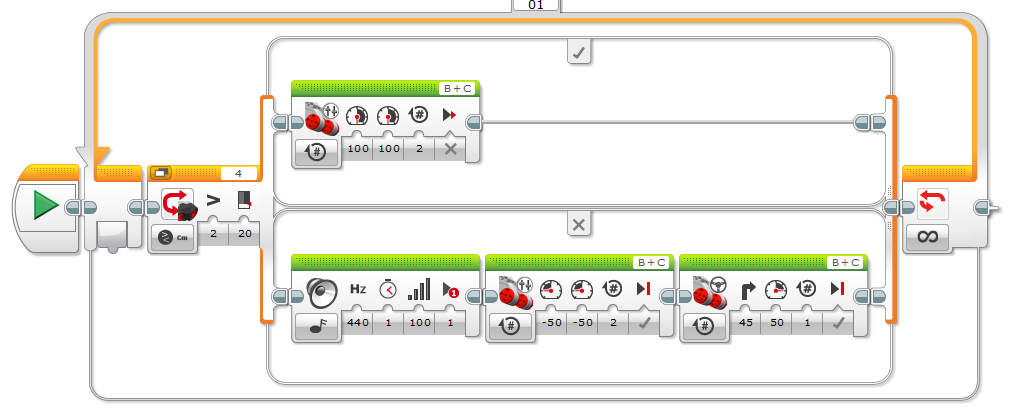
\includegraphics[width= 15cm]{Prog_Ultraschallsensor}
\caption{Lego-Programm zum Test und Kennenlernen des Ultraschallsensor}
\label{fig:ultraschallsensor}
\end{figure}
Im der Abbildung \vref{fig:ultraschallsensor} wird das, mit der Lego-Programmierumgebung erstellte, Programm dargestellt. 
\section{Testprogramm des Farbsensor}

